\documentclass[12pt]{article}
\usepackage[UTF8]{ctex}
\usepackage{geometry}
\usepackage{listings}
\usepackage{graphicx}
\usepackage{subfigure}
\usepackage{array}
\usepackage{caption}    
\usepackage{float}
\usepackage{subfloat}
\usepackage{hyperref}
\usepackage{bookmark}
\usepackage{amsmath}
\usepackage{url}
\usepackage{amsfonts,amssymb}

\geometry{left=15mm,right=15mm,top=20mm,bottom=20mm}
\title{期末项目报告\\ \large ——基于渐进式光子映射(SPPM)的图形渲染}

\author{PB21010410 高凡 \\PB21010362 汪兆辰}
\date{\today}
\newcommand{\upcite}[1]{\textsuperscript{\textsuperscript{\cite{#1}}}}

\begin{document}

\maketitle

\section{项目介绍}
\subsection{从基本全局光子映射(Basic Photon Mapping)讲起}
有效的实现全局光照(Global Illumination)的模拟是计算机图形学中的一个经典问题,在1998年Veach的博士论文中给出了无偏(unbiased)Monte-Carlo模拟的Path Tracing算法,但PT算法路径追踪在模拟散焦(caustics)时并不准确,同时
由于Monte-Carlo采样的误差阶是$\mathcal{O} (n^{-\frac{1}{2}})$,增加采样点对最终渲染结果的效果有限。

\begin{figure}[htbp]
    \centering
    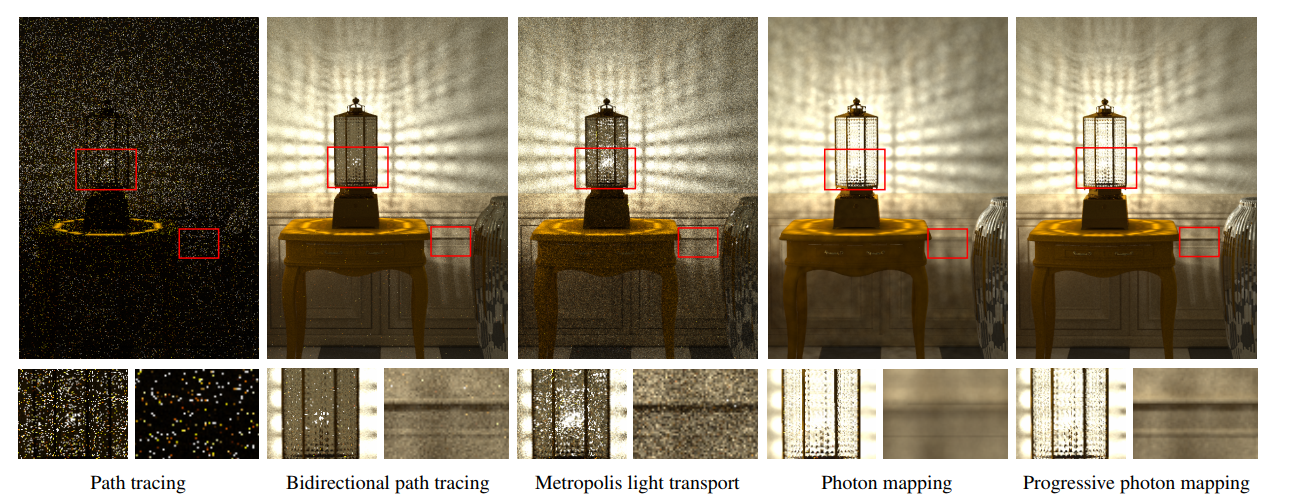
\includegraphics[scale=0.6]{pic1.png}
    \caption{几种光子映射算法的效果对比}
\end{figure}

对这种算法的一种改进是光子映射(Photon Mapping), 最朴素的光子映射分为两个阶段:第一个阶段需要构建一张光子贴图,用来存储从光源发射出的所有光子的通量信息;第二阶段从相机进行传统的路径追踪,在追踪到漫反射表面时统计附近的光子信息,并根据这些信息计算辐射率(radiance). 

\subsubsection{光子贴图}

构建光子贴图的基本思路是:让光源发出光子,并让光子在场景中反复弹射,直到被某个漫反射表面彻底吸收为止. 首先需要基于光源采样以确定光子的射线与初始功率,其中射线按照光源随机采样,而初始功率根据
\begin{equation}
    \Phi = \frac{L_e |\cos \theta|}{pdf_A (x)pdf_\omega (\omega)}
\end{equation}
来确定,其中$L_e$为光源自身的辐射率. 

在获得光子的初始状态后,需要对每一束光子在场景中反复迭代。当射线与表面相交时,按照表面的材质生成反射分布BSDF,并基于该BSDF记录下反射的方向与类型。如果反射类型为漫反射,就将光子的位置、路径与功率记录到光子贴图中,并随机按照反射比例判断是否终止迭代,如果未被吸收,则更新光子的功率,算法如下:

首先计算当前材质的反射率:
\begin{equation}
    R=\frac{f(x_{i-1}\rightarrow x_i \rightarrow x_{i+1})|\cos \theta|}{pdf_\omega (x_i \rightarrow x_{i+1})}
\end{equation}

然后得出光子的下一次功率:
\begin{equation}
    \Phi_{i+1}=\Phi_i \frac{R}{N_{BxDF}}
\end{equation}
其中$N_{BxDF}$为当前交点的反射分布下的反射模型的总数.

为了存储光子贴图,并加速光子映射,一种存储方式是按照光子图的位置构建平衡kd树,并用kNN算法进行优化,虽然建树的时间略微增加,但这种方式可以将后续查询的时间复杂度降到$\mathcal{O}(\sqrt{N}+K)$.

\subsubsection{基本全局光子映射}

由渲染方程:
\begin{equation}
    L_r(x,\omega)=\int_\Omega f(x,\omega',\omega)L_i(x,\omega')|\cos \theta'|d\omega'
\end{equation}
将辐射率
\begin{equation}
    L_i(x,\omega')=\frac{d^2 \Phi_i(x,\omega')}{dA|\cos \theta'|d\omega'}
\end{equation}
代入渲染方程得:
\begin{align}
    L_r(x,\omega)&=\int_\Omega f(x,\omega,\omega')\frac{d^2 \Phi_i(x,\omega')}{dA|\cos \theta'|d\omega'}|\cos \theta'|d\omega'\\
    &=\int _\Omega f(x,\omega,\omega')\frac{d^2\Phi_i(x,\omega')}{dA}
\end{align}
将其离散化得到:
\begin{equation}
    L_r(x,\omega)=\sum_{p=1}^{N}f(x,\omega_p,\omega)\frac{\Delta \Phi_p(x_p,\omega_p)}{\Delta A}
\end{equation}
其中$\Phi_p,\omega_p$分别为光子的功率与方向.

利用kd树和上述公式,取定合适的N就可以得到$L_r$, 样本N数量越多,估算的结果越接近真实值. 而由kd树的kNN算法可以得到样本所占的面积$\Delta A$,其中半径为
\begin{equation}
    r=\max(Dist(x,x_1),Dist(x,x_2),\ldots ,Dist(x,x_N))
\end{equation}

\subsubsection{全局光子映射的局限性}
作为最原始的光子映射方案,全局光子映射保留了相当明显的光子映射特征:由于样本的随机性与密度估计的插值效应,在样本较少的情况下,光子映射会出现明显的块状斑点(如图1-4).
另一方面,当场景中的大多数表面为光滑材质时,第一阶段中生成光子贴图需要多次迭代才能使得光子最终被吸收,而单纯为迭代次数设置上限会使得图像整体偏暗,需要更好的改进办法.

\begin{figure}[htbp]
    \centering
    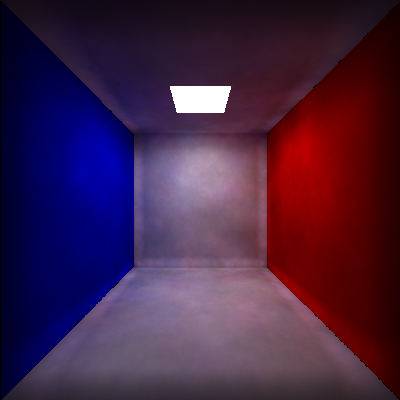
\includegraphics[scale=0.6]{pic2.png}
    \caption{全局光子映射渲染效果}
\end{figure}
其次,如图2所示,全局光子映射在场景的墙角处有明显的渗色情况,出现这种情况的原因是在密度估计过程中样本数量取的过大,使得部分与被估计光子不在同一平面的光子也参与了估计。在不占用大量内存与渲染时间的前提下很难有效果较好的优化,
所以需要对算法进一步改进。

\subsection{随机渐进式光子映射(SPPM)}
SPPM在PM的基础上调整了计算的模型,使得计算的结果可以近似完全收敛。首先要从PM过渡到渐进式光子映射(PPM),将PM中单次的光子映射改为多次光子映射并叠加,实现渐进式的收敛;之后再进一步将射线追踪阶段也拆为多次,并将PPM中基于场景的计算方式改为基于像素计算,以获得更低的开销与更快的收敛速度。

\subsubsection{从PM到PPM}
在\cite{7}中,Jensen提出了一种改进措施,将PM的光子映射拆成多次,形成多张光子图并分批执行密度估计,对所有结果取平均值,但这最多将估计范围收敛到对应的kNN范围r内,而如果一开始将r取的很小,会使得估计范围内光子密度很低,降低估计效率,所以
实现对估计半径r的控制成为了重点的问题。

改进方案的前几步与Jensen 2004相同:假设第一次密度估计需要$N_1(x)$个光子,在第一轮密度估计后,利用kNN算法可以得到估计范围的半径$R_1(x)$,并得到第一次估计的密度$d_1(x)=\frac{N_1(x)}{\pi R_1(x)^2}$.之后维持半径$R_1(x)$不变,重新生成一张光子图,并围绕新的光子图基于同样的半径$R_1(x)$做一次密度估计,假设新的光子数目为$M_1(x)$,
则新的密度估计为
\begin{equation}
    d_2(x)=\frac{N_1(x)+M_1(x)}{\pi R_1(x)^2}
\end{equation}


在进行下一步密度估计之前,先对估计半径进行收缩,假设在收缩过程中密度是不变的,可以计算出半径缩减后下一轮光子个数$N_2(x)$与密度$d_2(x)$的关系:
\begin{equation}
    d_2(x)=\frac{N_2(x)}{\pi R_2(x)^2}=\frac{N_2(x)}{\pi (R_1(x)-\Delta R_1(x))^2}
\end{equation}
其中$\Delta R_1(x)$为第一次迭代过渡到第二次过程中半径的缩减量.而下一轮光子数量$N_2(x)$取决于上一轮光子$N_1(x)$与新增光子$M_1(x)$,这里$N_1(x)$无法更改,但可以控制新增部分的比例,即
\begin{equation}
    N_2(x)=N_1(x)+\alpha M_1(x)
\end{equation}
其中缩减系数$\alpha$实际上控制了半径$R_2(x)$的衰减速度.结合(10)-(12)三式,可得:
\begin{equation}
    R_2(x)=R_1(x) \sqrt{\frac{N_1(x)+\alpha M_1(x)}{N_1(x)+M_1(x)}}
\end{equation}
重复此过程,可以使得估算半径不断收敛。

记x处出射到相机方向$\omega$的总通量为:
\begin{equation}
    \tau(x,\omega):=\sum_{p=1}^{N} f(x,\omega_p,\omega)\Delta \Phi_p(x,\omega_p) 
\end{equation}
假设已经迭代了i轮,累积了$N_i(x)$个光子,那么这些光子的总通量理论上可以计算为:
\begin{equation}
    \tau_i(x,\omega)=\sum_{p=1}^{N_i(x)} f(x,\omega_p,\omega)\Delta \Phi_p(x,\omega_p)
\end{equation}
然后下一步,缩减前新增$M_i(x)$个光子,尽管由于半径缩减最终只保留其中的一部分,但依然需要计算全部新增光子的总通量,记为: 
\begin{equation}
    \phi_i(x,\omega)=\sum_{p=1}^{M_i(x)} f(x,\omega_p,\omega)\Delta \Phi_p(x,\omega_p)
\end{equation}
由公式(13)可以计算出收敛后半径:
\begin{equation}
    R_{i+1}(x)=R_i(x)\sqrt{\frac{N_i(x)+\alpha M_i(x)}{N_i(x)+M_i(x)}}
\end{equation}
并估计出缩减后保留的总通量:
\begin{equation}
    \tau_{i+1}(x,\omega)=(\tau_i(x,\omega)+\phi_i(x,\omega))\frac{N_i(x)+\alpha M_i(x)}{N_i(x)+M_i(x)}
\end{equation}
结合式(8)可以计算出第i+1轮的辐射率:
\begin{align}
    L_r(x,\omega)&=\frac{1}{\Delta A}\sum_{p=1}^{N_{i+1}(x)}f(x,\omega_p,\omega)\Delta \Phi_p(x,\omega_p)\\
    &=\frac{1}{\pi R_{i+1}(x)^2}\frac{\tau_{i+1}(x,\omega)}{N_e(i+1)}
\end{align}
随着迭代次数不断增大,总通量$\tau_{i+1}(x,\omega)$增大,密度估计半径$R_{i+1}(x)$缩小,全局光子总数$N_e(i+1)$越来越多,能够完全收敛。

但由于PPM需要为每个像素点分配很多射线与漫反射面相交形成的命中点才能有效去噪,仍然需要较大的内存开销。
\subsubsection{从PPM到SPPM}
SPPM在PPM的基础上改进了对命中点的生成,在每个渲染阶段,先进行一次射线追踪,再对每次射线追踪生成一小批命中点,并围绕这些命中点在一个像素范围内抖动更新,从而当样本量足够大时,估算的即为像素内的全部区域。
而SPPM的计算公式与PPM的式(20)只需将命中点x改为像素区域S:
\begin{equation}
    L_r(S,\omega)=\frac{1}{\pi R_{i+1}(S)^2}\frac{\tau_{i+1}(S,\omega)}{N_e(i+1)}
\end{equation}

\section{代码介绍}



\section{效果展示}


\begin{thebibliography}{3}
    \bibitem{1} \url{https://zhuanlan.zhihu.com/p/208356944}
    \bibitem{2} \url{https://zhuanlan.zhihu.com/p/259565623}
    \bibitem{3} \url{https://graphics.stanford.edu/courses/cs348b-00}
    \bibitem{4} M.Pharr, W.Jakob, and G.Humphreys. Physically Based Rendering: From Theory To Implementation. 2018.
    \bibitem{5} T.Hachisuka, S.Ogaki, and H.W.Jensen. Progressive Photon Mapping. ACM SIGGRAPH Asia 2008 Papers, 2008.
    \bibitem{6} T.Hachisuka, H.W.Jensen. Stochastic progressive photon mapping. ACM Transactions on Graphics, 2009.
    \bibitem{7} H.W.Jensen. ACM SIGGRAPH 2004 Course Notes. A practical guide to global illumination using ray tracing and photon mapping, 2004.
    \bibitem{8} E.Veach. Stanford University. Robust monte carlo methods for light transport simulation, 1998.
\end{thebibliography}

\end{document}